\documentclass[aspectratio=169]{beamer}

\usepackage[utf8]{inputenc}
\usepackage{graphicx}
\usepackage{tcolorbox}
\usepackage{caption}
\usepackage{subcaption}
\usepackage{tikz}
\usetikzlibrary{positioning}
\usepackage[export]{adjustbox}

\usefonttheme{professionalfonts}
\usetikzlibrary{intersections,patterns}

\usepackage{pifont}
\definecolor{donegreen}{RGB}{0,120,60}
\definecolor{plannedorange}{RGB}{200,110,0}

\newcommand{\done}{{\color{donegreen}\ding{51}}}      % ✓
\newcommand{\planned}{{\color{plannedorange}\ding{108}}} % ○ tick (planned)

% Bibliography (keep if you actually cite in slides)
\usepackage[style=phys]{biblatex}
\addbibresource{hello.bib}

% -----------------------------
% Theme + professional green
% -----------------------------
\usetheme{Madrid}
\definecolor{ucdgreen}{RGB}{0, 102, 51} % dark green
\usecolortheme[named=ucdgreen]{structure}
\setbeamertemplate{navigation symbols}{}

% -----------------------------
% Title metadata (fix first slide)
% -----------------------------
\title[Research Studies Panel 1]{Research Studies Panel 1}
\author[Lainey Ward]{Lainey Ward}
\institute[]{Decarb-AI Centre, School of Civil Engineering\\
Primary supervisor: Dr Fiachra O’Loughlin \\ Co-supervisor: Dr Conor Sweeney}
\date[16 March 2026]{16 March 2026}

\begin{document}

% Title slide
\begin{frame}
  \titlepage
\end{frame}

% Overview
\begin{frame}{Overview}
    \begin{itemize}
        \item Research Overview
        \item Ongoing Research
        \item Future Plan
        \item Training \& Development
    \end{itemize}
\end{frame}

% Project overview (fix slide content + add venn on right)
\begin{frame}{Research Overview}
    \begin{columns}[T,totalwidth=\textwidth]
        \begin{column}{0.56\textwidth}
            
            \vspace{0.2em}
            \textbf{Motivations \& Gaps}
            \begin{itemize}
                \item Operational importance of the S2S range
                \item Verification focused on single variables, not multi-hazard events
                \item Teleconnection-conditioned predictability largely unexplored
            \end{itemize}
            
            \vspace{2em}
            \textit{How does  S2S forecast skill vary for multi-hazard
            weather events, and under which large-scale atmospheric
            states does this skill emerge?}
        \end{column}

        \begin{column}{0.44\textwidth}
            \centering
            % Simple 3-set Venn diagram in TikZ (edit labels as needed)
            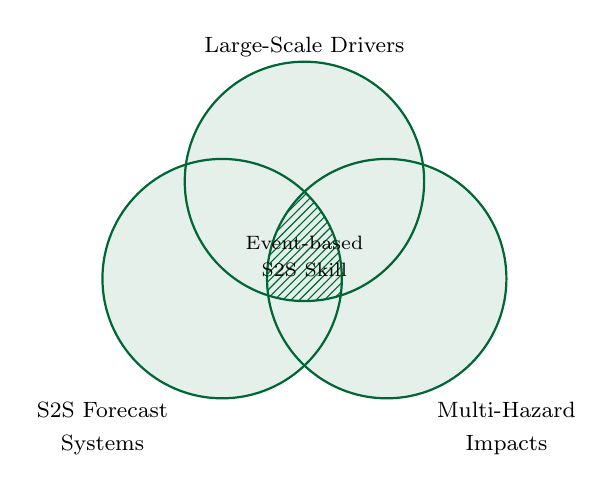
\begin{tikzpicture}[scale=0.95]
            \def\r{1.6}
            
            % Define circles
            \path[name path=A] (-1.1,0) circle (\r);
            \path[name path=B] ( 1.1,0) circle (\r);
            \path[name path=C] (0,1.3) circle (\r);
            
            % Light fill
            \fill[ucdgreen!10] (-1.1,0) circle (\r);
            \fill[ucdgreen!10] ( 1.1,0) circle (\r);
            \fill[ucdgreen!10] (0,1.3) circle (\r);
            
            % Outline
            \draw[ucdgreen, thick] (-1.1,0) circle (\r);
            \draw[ucdgreen, thick] ( 1.1,0) circle (\r);
            \draw[ucdgreen, thick] (0,1.3) circle (\r);
            
            % Hatched triple intersection
            \begin{scope}
              \clip (-1.1,0) circle (\r);
              \clip ( 1.1,0) circle (\r);
              \clip (0,1.3) circle (\r);
              \fill[pattern=north east lines, pattern color=ucdgreen] (-2,-2) rectangle (2,3);
            \end{scope}
            
            % Labels inside circles
            \node[align=center] at (-2.7,-2.0) {\footnotesize S2S Forecast \\ \footnotesize Systems};
            \node[align=center] at ( 2.7,-2.0) {\footnotesize Multi-Hazard\\ \footnotesize Impacts};
            \node[align=center] at (0,3.1) {\footnotesize Large-Scale Drivers};
            
            % Centre text
            \node[align=center] at (0,0.3)
            {\scriptsize Event-based\\[-0.2em]\scriptsize S2S Skill};
            
            \end{tikzpicture}

            \vspace{0.4em}
            \captionof{figure}{Conceptual framework}
        \end{column}
    \end{columns}
\end{frame}

\begin{frame}{Ongoing research}
    \begin{itemize}
        \item Operational S2S reforecast datasets acquired and processed
        \item Unified forecast–reanalysis verification framework implemented
        \item Deterministic seasonal skill evaluated across leads and seasons
        \item Baseline predictability characteristics established for Ireland
    \end{itemize}
\end{frame}

\begin{frame}{Deterministic Seasonal Skill}

\begin{columns}[T,totalwidth=\textwidth]

\begin{column}{0.49\textwidth}
    \centering
    \includegraphics[height=0.6\textheight,keepaspectratio]{figures/acc_leadtime.pdf}
    
    \vspace{0.3em}
    {\footnotesize ACC across lead times.}
\end{column}

\begin{column}{0.49\textwidth}
    \centering
    \includegraphics[height=0.6\textheight,keepaspectratio]{figures/rmse_leadtime.pdf}
    
    \vspace{0.3em}
    {\footnotesize RMSE across lead times.}
\end{column}

\end{columns}

\end{frame}

\begin{frame}{Future Plan}
    \begin{itemize}
        \item Multi-hazard index development
        \item Flood–drought / drought–flood transitions
        \item Event-based S2S verification
        \item Probabilistic skill assessment
        \item Circulation-conditioned skill
        \item EMS abstract + first manuscript
    \end{itemize}
\end{frame}

% FINAL SLIDE
\begin{frame}{Training \& Development}
\small

\textbf{Credits}
\begin{itemize}
    \setlength{\itemsep}{1pt}
    \item ACM41070 (5) \done \quad + STAT41130 (5) \done \quad 
          + STAT40700 (5) \planned \quad 
          + RPL (15) \planned \quad = 30
\end{itemize}

\vspace{0.4em}

\begin{columns}[T,totalwidth=\textwidth]

% -------- RIGHT COLUMN --------
\begin{column}{0.52\textwidth}
\textbf{Conferences \& Meetings}
\begin{itemize}
    \setlength{\itemsep}{1pt}
    \item Irish SIAM–IMS Student Conference \done
    \item EMS Annual Meeting \planned
    \item ANTICIPATE COST Action: \planned
    \begin{itemize}
        \setlength{\itemsep}{1pt}
        \item Working Group Meeting (Switzerland)
        \item Short-Term Scientific Mission
        \item COST Summer School 
    \end{itemize}
\end{itemize}
\end{column}

\hspace{0.04\textwidth}  % adjust this value

% -------- LEFT COLUMN --------
\begin{column}{0.48\textwidth}
\textbf{Training}
\begin{itemize}
    \setlength{\itemsep}{1pt}
    \item Research Integrity Training \done
    \item Sonic HPC Training \done
    \item DestinE – ML for Earth Systems \planned
    \item IFI iScholar Programme \planned
\end{itemize}
\end{column}

\end{columns}

\vspace{0.4em}

\textbf{Other}
\begin{itemize}
    \setlength{\itemsep}{1pt}
    \item First-author submission to \textit{Remote Sensing}
    \item SOM Rep.
\end{itemize}

\end{frame}

\end{document}